\documentclass[10pt,a4paper,twoside]{article}\usepackage[]{graphicx}\usepackage[]{xcolor}
% maxwidth is the original width if it is less than linewidth
% otherwise use linewidth (to make sure the graphics do not exceed the margin)
\makeatletter
\def\maxwidth{ %
  \ifdim\Gin@nat@width>\linewidth
    \linewidth
  \else
    \Gin@nat@width
  \fi
}
\makeatother

\definecolor{fgcolor}{rgb}{0.345, 0.345, 0.345}
\newcommand{\hlnum}[1]{\textcolor[rgb]{0.686,0.059,0.569}{#1}}%
\newcommand{\hlstr}[1]{\textcolor[rgb]{0.192,0.494,0.8}{#1}}%
\newcommand{\hlcom}[1]{\textcolor[rgb]{0.678,0.584,0.686}{\textit{#1}}}%
\newcommand{\hlopt}[1]{\textcolor[rgb]{0,0,0}{#1}}%
\newcommand{\hlstd}[1]{\textcolor[rgb]{0.345,0.345,0.345}{#1}}%
\newcommand{\hlkwa}[1]{\textcolor[rgb]{0.161,0.373,0.58}{\textbf{#1}}}%
\newcommand{\hlkwb}[1]{\textcolor[rgb]{0.69,0.353,0.396}{#1}}%
\newcommand{\hlkwc}[1]{\textcolor[rgb]{0.333,0.667,0.333}{#1}}%
\newcommand{\hlkwd}[1]{\textcolor[rgb]{0.737,0.353,0.396}{\textbf{#1}}}%
\let\hlipl\hlkwb

\usepackage{framed}
\makeatletter
\newenvironment{kframe}{%
 \def\at@end@of@kframe{}%
 \ifinner\ifhmode%
  \def\at@end@of@kframe{\end{minipage}}%
  \begin{minipage}{\columnwidth}%
 \fi\fi%
 \def\FrameCommand##1{\hskip\@totalleftmargin \hskip-\fboxsep
 \colorbox{shadecolor}{##1}\hskip-\fboxsep
     % There is no \\@totalrightmargin, so:
     \hskip-\linewidth \hskip-\@totalleftmargin \hskip\columnwidth}%
 \MakeFramed {\advance\hsize-\width
   \@totalleftmargin\z@ \linewidth\hsize
   \@setminipage}}%
 {\par\unskip\endMakeFramed%
 \at@end@of@kframe}
\makeatother

\definecolor{shadecolor}{rgb}{.97, .97, .97}
\definecolor{messagecolor}{rgb}{0, 0, 0}
\definecolor{warningcolor}{rgb}{1, 0, 1}
\definecolor{errorcolor}{rgb}{1, 0, 0}
\newenvironment{knitrout}{}{} % an empty environment to be redefined in TeX

\usepackage{alltt}

%%% Load some LaTeX packages:
\usepackage[utf8]{inputenc}
\usepackage[nottoc]{tocbibind}      % for bibliography in the table of contents
\usepackage{hyperref}                      % link to website: \url{}.
\usepackage[hang,footnotesize,bf]{caption} % customized caption
\usepackage{amsmath}                       % for mathematical features 
\usepackage[left=2.5cm,top=3cm,bottom=3cm,right=2.5cm]{geometry}   % text margins
\usepackage{booktabs}                      % for booktabs in print(xtable)).
\usepackage{authblk}                       % for footnote style author/affiliation
\usepackage{parskip}
\usepackage{dsfont}
\usepackage{amssymb}
\usepackage{mathtools}
\usepackage{graphicx}
\usepackage{multirow}
\usepackage{float}
\usepackage{caption}
\usepackage{cancel}
\usepackage{nccmath}
\usepackage{geometry}
\usepackage{amsfonts} 
\usepackage{bbm}
\floatplacement{figure}{H}




%%% Some LaTeX "macros":
\newcommand{\R}{\textsf{R}}
\newcommand{\Rpackage}[1]{\textsf{#1}}
\newcommand{\Robject}[1]{\texttt{#1}}
\newcommand*{\QEDB}{\null\nobreak\hfill\ensuremath{\blacksquare}}







\IfFileExists{upquote.sty}{\usepackage{upquote}}{}
\begin{document}


\begin{titlepage}
  \begin{center}
  %{\includegraphics[width=0.5\textwidth]{logo}\par}
  %\vspace{1cm}
  \LARGE
  {Universitat Aut\`{o}noma de Barcelona \par}
  
  \vspace{1cm}
  
  \Large
  \scshape{Facultat de Ci\`{e}ncies \par}
  
  \vspace{3cm}
  
  \Huge
  \bfseries{{Assignment 2 \par}}
  
  \vspace{1cm}
  
  \Huge
  \scshape{Missing data in linear regression models \par}
  \vfill
  
  \vspace{2cm}
  
  \Large
  \scshape{Statistics in Health Sciences \par}
  \vfill
  
  \vspace{2cm}
  

  \Large
  {Sergi Cant\'{o}n Sim\'{o} - 1569251 \par}
  \Large
  {C\`{e}lia Mart\'{i}nez Frago - 1569504 \par}
  \Large 
  {Goretti Pena Lorente - 1566866 \par}
  \Large 
  {Guillermo Raya Garc\'{i}a - 1568864 \par}
  
  \Large 
  {Assignment identifier: A2 \par}
  
  \Large 
  {Group identifier: G04 \par}
  
  \vspace{1cm}
  \Large
  {8/12/2022 \par}
  
  \vfill
  \date{}
  
  \end{center}
\end{titlepage}

%\maketitle

%\thispagestyle{empty}


%%%%%%%%%%%%%%%
%%%
%%% Table of contents
%%%
%%%%%%%%%%%%%%%
\clearpage
\tableofcontents
\clearpage

\pagenumbering{arabic}



%%%%%%%%%%%%%%%
%%%
%%% Section: Introduction
%%%
%%%%%%%%%%%%%%%
\section{Introduction}
\label{sec:intro}
In 1961, Doll and Hill\cite{ref1} sent out a questionnaire to all men on the British Medical Register asking about their smoking habits. Almost $70\%$ of such men replied. Death certificates were obtained for medical practitioners and causes of death were assigned on the basis of these certificates. The \Robject{breslow} data set\cite{ref2} (attached in the \Robject{breslow.RData} file) contains the person-years of observations and deaths from coronary artery disease accumulated during the first ten years of the study. Such data are shown in Table \ref{tab:table1}.



\begin{table}[h]
\centering
\begin{tabular}{crrrrrr}
\toprule
\multicolumn{1}{c}{ } & \multicolumn{2}{c}{Person-years} & \multicolumn{2}{c}{Coronary deaths} \\
\cmidrule(l{3pt}r{3pt}){2-3} \cmidrule(l{3pt}r{3pt}){4-5}
Age & Nonsmokers & Smokers & Nonsmokers & Smokers \\
\midrule
35-44 & 18790 & 52407  & 2 & 32\\
45-54 & 10673 & 43248  & 12 & 104\\
55-64 & 5710 & 28612  & 28 & 206\\
65-74 & 2585 & 12663  & 28 & 186\\
75-84 & 1462 & 5317 & 31 & 102\\
\bottomrule
\end{tabular}
\caption{Data on coronary death rates.}
\label{tab:table1}
\end{table}

The aim of this exercise is to analyze the relationship between incidence of coronary deaths and both smoke status (exposure of interest) and age (as a potential confounder).


%%%%%%%%%%%%%%%
%%%
%%% Section: Comparing incidence rates
%%%
%%%%%%%%%%%%%%%
\section{Comparing incidence rates}
\label{sec:Comparing_incidence_rates}
\begin{enumerate}
  \item Add extra columns in Table \ref{tab:table1} for:
  \begin{enumerate}
    \item $I_{r_{ij}}$, the sample coronary death rates per 1000 person-years for smoke status $i$ ($i = 0$ for nonsmokers and $i = 1$ for smokers) and age group $j$ ($j = 0, 1, ...,4$) for 35-44, 45-54, ..., 75-84, respectively)\footnote{\label{note1}See Appendix \ref{app:Ir and IRR}.} (two columns).

    \item $IRR_{j} = \frac{I_{r_{1j}}}{I_{r_{0j}}}$, the incidence rate ratio for smokers vs. nonsmokers for the age group $j$ \footref{note1} (one column).

  \end{enumerate}
  Print the update table as Table 2, with a proper caption.
  
\begin{kframe}
\begin{alltt}
\hlstd{> }\hlstd{Age} \hlkwb{=} \hlkwd{c}\hlstd{(Data}\hlopt{$}\hlstd{age[}\hlnum{1}\hlstd{], Data}\hlopt{$}\hlstd{age[}\hlnum{2}\hlstd{], Data}\hlopt{$}\hlstd{age[}\hlnum{3}\hlstd{], Data}\hlopt{$}\hlstd{age[}\hlnum{4}\hlstd{], Data}\hlopt{$}\hlstd{age[}\hlnum{5}\hlstd{])}
\hlstd{> }\hlstd{Nonsmokers_Py} \hlkwb{=} \hlkwd{c}\hlstd{(Data}\hlopt{$}\hlstd{personYears[}\hlnum{1}\hlstd{], Data}\hlopt{$}\hlstd{personYears[}\hlnum{2}\hlstd{],}
\hlstd{+ }                  \hlstd{Data}\hlopt{$}\hlstd{personYears[}\hlnum{3}\hlstd{],Data}\hlopt{$}\hlstd{personYears[}\hlnum{4}\hlstd{], Data}\hlopt{$}\hlstd{personYears[}\hlnum{5}\hlstd{])}
\hlstd{> }\hlstd{Smokers_Py} \hlkwb{=} \hlkwd{c}\hlstd{(Data}\hlopt{$}\hlstd{personYears[}\hlnum{6}\hlstd{], Data}\hlopt{$}\hlstd{personYears[}\hlnum{7}\hlstd{],}
\hlstd{+ }               \hlstd{Data}\hlopt{$}\hlstd{personYears[}\hlnum{8}\hlstd{],Data}\hlopt{$}\hlstd{personYears[}\hlnum{9}\hlstd{], Data}\hlopt{$}\hlstd{personYears[}\hlnum{10}\hlstd{])}
\hlstd{> }\hlstd{Nonsmokers_Cd} \hlkwb{=} \hlkwd{c}\hlstd{(Data}\hlopt{$}\hlstd{deaths[}\hlnum{1}\hlstd{], Data}\hlopt{$}\hlstd{deaths[}\hlnum{2}\hlstd{],}
\hlstd{+ }                  \hlstd{Data}\hlopt{$}\hlstd{deaths[}\hlnum{3}\hlstd{], Data}\hlopt{$}\hlstd{deaths[}\hlnum{4}\hlstd{],Data}\hlopt{$}\hlstd{deaths[}\hlnum{5}\hlstd{])}
\hlstd{> }\hlstd{Smokers_Cd} \hlkwb{=} \hlkwd{c}\hlstd{(Data}\hlopt{$}\hlstd{deaths[}\hlnum{6}\hlstd{], Data}\hlopt{$}\hlstd{deaths[}\hlnum{7}\hlstd{], Data}\hlopt{$}\hlstd{deaths[}\hlnum{8}\hlstd{],}
\hlstd{+ }               \hlstd{Data}\hlopt{$}\hlstd{deaths[}\hlnum{9}\hlstd{],Data}\hlopt{$}\hlstd{deaths[}\hlnum{10}\hlstd{])}
\hlstd{> }\hlstd{Nonsmokers_Ir} \hlkwb{=} \hlkwd{c}\hlstd{(Ir_Nonsmokers[}\hlnum{1}\hlstd{], Ir_Nonsmokers[}\hlnum{2}\hlstd{], Ir_Nonsmokers[}\hlnum{3}\hlstd{],}
\hlstd{+ }                  \hlstd{Ir_Nonsmokers[}\hlnum{4}\hlstd{], Ir_Nonsmokers[}\hlnum{5}\hlstd{])}
\hlstd{> }\hlstd{Smokers_Ir} \hlkwb{=} \hlkwd{c}\hlstd{(Ir_smokers[}\hlnum{1}\hlstd{], Ir_smokers[}\hlnum{2}\hlstd{], Ir_smokers[}\hlnum{3}\hlstd{],}
\hlstd{+ }               \hlstd{Ir_smokers[}\hlnum{4}\hlstd{], Ir_smokers[}\hlnum{5}\hlstd{])}
\hlstd{> }\hlstd{IRR_list} \hlkwb{=} \hlkwd{c}\hlstd{(IRR[}\hlnum{1}\hlstd{], IRR[}\hlnum{2}\hlstd{], IRR[}\hlnum{3}\hlstd{], IRR[}\hlnum{4}\hlstd{], IRR[}\hlnum{5}\hlstd{])}
\hlstd{> }\hlstd{data} \hlkwb{=} \hlkwd{data.frame}\hlstd{(Age, Nonsmokers_Py, Smokers_Py, Nonsmokers_Cd, Smokers_Cd,}
\hlstd{+ }                  \hlstd{Nonsmokers_Ir, Smokers_Ir, IRR_list)}
\hlstd{> }
\hlstd{> }
\hlstd{> }\hlkwd{kable}\hlstd{(data,} \hlstr{'latex'}\hlstd{,} \hlkwc{booktabs} \hlstd{= T,} \hlkwc{row.names} \hlstd{=} \hlnum{NA}\hlstd{,}
\hlstd{+ }  \hlkwc{col.names} \hlstd{=} \hlkwd{c}\hlstd{(}\hlstr{'Age'}\hlstd{,} \hlstr{'Nonsmokers'}\hlstd{,} \hlstr{'Smokers'}\hlstd{,}
\hlstd{+ }                \hlstr{'Nonsmokers'}\hlstd{,} \hlstr{'Smokers'}\hlstd{,}
\hlstd{+ }                \hlstr{'Nonsmokers'}\hlstd{,} \hlstr{'Smokers'}\hlstd{,} \hlstr{'Incidence Rate Ratio'}\hlstd{),}
\hlstd{+ }  \hlkwc{caption} \hlstd{=} \hlstr{'Data on coronary death rates including incidence 
  rate depending on somke status and incidence rate ratio.'}\hlstd{)} \hlopt
\hlstd{+ }  \hlkwd{kable_styling}\hlstd{(}\hlkwc{latex_options} \hlstd{=} \hlstr{"HOLD_position"}\hlstd{)} \hlopt
\hlstd{+ }  \hlkwd{add_header_above}\hlstd{(}\hlkwd{c}\hlstd{(}\hlstr{" "} \hlstd{=} \hlnum{1}\hlstd{,}
\hlstd{+ }  \hlstr{"Person-years"} \hlstd{=} \hlnum{2}\hlstd{,}
\hlstd{+ }  \hlstr{"Coronary deaths"} \hlstd{=} \hlnum{2}\hlstd{,}
\hlstd{+ }  \hlstr{"Incidence rate"} \hlstd{=} \hlnum{2}\hlstd{,}
\hlstd{+ }  \hlstr{" "} \hlstd{=} \hlnum{1}\hlstd{))}
\end{alltt}
\end{kframe}\begin{table}[H]

\caption{\label{tab:table2}Data on coronary death rates including incidence 
  rate depending on somke status and incidence rate ratio.}
\centering
\begin{tabular}[t]{lrrrrrrr}
\toprule
\multicolumn{1}{c}{ } & \multicolumn{2}{c}{Person-years} & \multicolumn{2}{c}{Coronary deaths} & \multicolumn{2}{c}{Incidence rate} & \multicolumn{1}{c}{ } \\
\cmidrule(l{3pt}r{3pt}){2-3} \cmidrule(l{3pt}r{3pt}){4-5} \cmidrule(l{3pt}r{3pt}){6-7}
Age & Nonsmokers & Smokers & Nonsmokers & Smokers & Nonsmokers & Smokers & Incidence Rate Ratio\\
\midrule
35-44 & 18790 & 52407 & 2 & 32 & 0.11 & 0.61 & 5.7\\
45-54 & 10673 & 43248 & 12 & 104 & 1.12 & 2.40 & 2.1\\
55-64 & 5710 & 28612 & 28 & 206 & 4.90 & 7.20 & 1.5\\
65-74 & 2585 & 12663 & 28 & 186 & 10.83 & 14.69 & 1.4\\
75-84 & 1462 & 5317 & 31 & 102 & 21.20 & 19.18 & 0.9\\
\bottomrule
\end{tabular}
\end{table}


  
  \item For age group 45-54, complete the following sentences with numbers and proper units \textbf{(using} \verb+\Sexpr+ \textbf{in your \Robject{Rnw} document)}\footnote{See Appendix \ref{app:IncidenceRates2}.}:

  \begin{enumerate}
    \item The incidence rate among smokers was 2.4 coronary deaths a year per 1000 people.
    \item The incidence rate among nonsmokers was 1.12 coronary deaths a year per 1000 people.
    \item The incidence rate ratio was 2.14.
    \item The $p$-value of the Wald test to decide if the incidence rate among smokers is the same than among nonsmokers was 0.01.
    \item Write a paragraph for the interpretation of previous results (including all quantities):

      Observing the incidence rate for the age range of 45 to 54 years old, we can see that there were more cases of coronary deaths among the exposed group (roughly 2.4 cases a year per 1000 people, to be specific) than among the unexposed or "control" group (which suffered approximately 1.12 cases a year per 1000 people). Comparing the two values, we see that the smokers had an incidence rate nearly 2.14 times as big as non-smokers, a number that seems to indicate that smokers in this age group had a bigger chance of suffering from coronary death. In order to check if these results are significant, we have performed a Wald test (the null hypothesis being "the incidence rate of exposed and non-exposed groups are equivalent"), which estimated an approximate p-value of 0.01. Having received a p-value lower than our threshold of 0.05, we believe that the null hypothesis can be rejected: the test suggests that smoking could be associated with an increased incidence rate of coronary death among our selected demographic.

  \end{enumerate}
  \item For age group 75-84, complete the following sentences with numbers and proper units \textbf{(using} \verb+\Sexpr+ \textbf{in your \Robject{Rnw} document)}\footnote{See Appendix \ref{app:IncidenceRates3}.}:

  \begin{enumerate}
    \item The incidence rate among smokers was 19.18 coronary deaths a year per 1000 people.
    \item The incidence rate among nonsmokers was 21.2 coronary deaths a year per 1000 people
    \item The incidence rate ratio was 0.9.
    \item The \textit{p}-value of the Wald test to decide if the incidence rate among smokers is the same than among nonsmokers was 0.63.
    \item Write a paragraph for the interpretation of previous results (including all quantities).

    Observing the incidence rate for the age range of 75 to 84 years old, we can see that there were less cases of coronary deaths among the exposed group (roughly 19.18 cases a year per 1000 people, to be specific) than among the unexposed or "control" group (which suffered approximately 21.2 cases a year per 1000 people). Comparing the two values, we see that the smokers had an incidence rate about 0.9 times as big as non-smokers, a number that seems to indicate that smokers in this age group had a smaller chance of suffering from coronary death. In order to check if these results are significant, we have performed a Wald test (the null hypothesis being "the incidence rate of exposed and non-exposed groups are equivalent"), which estimated an approximate p-value of 0.63. Having received such a large p-value (way over our threshold of 0.05), we believe that the null hypothesis cannot be rejected with certainty: although our data shows that less individuals in the selected demographic suffered from coronary death, it seems too likely that these results were achieved by chance, and thus we could not conclude that smoking had a clear association with the risk of coronary death in this situation.
    
  \end{enumerate}
  \item Create a figure, named Figure \ref{fig:IRR_plot}, as follows:
  \begin{enumerate}
    \item Figure \ref{fig:IRR_plot} must include two plots, one of them on the left and another on the right. \textbf{Hint:} Use \Robject{par(mfrow = c(1, 2), ...)}.
    \item Both plots must represent age groups in the horizontal axis and rate ratios in the vertical axis.
    \item The plot on the right must represent the rate ratios in logarithmic scale. \textbf{Hint:} Use \Robject{plot(log = "y", ...)}.
    \item Both plots must include proper labels in both axes and proper ticks labels (for instance, horizontal axis must show labels 35-44, 45-54, ...). \textbf{Hint:} Use \Robject{plot(xaxt = "n", ...)} and then use \Robject{axis(1, at = ..., labels = ...)}.
    \item Figure \ref{fig:IRR_plot} must include a detailed caption.
  \end{enumerate}
\begin{knitrout}\footnotesize
\definecolor{shadecolor}{rgb}{0.969, 0.969, 0.969}\color{fgcolor}\begin{figure}
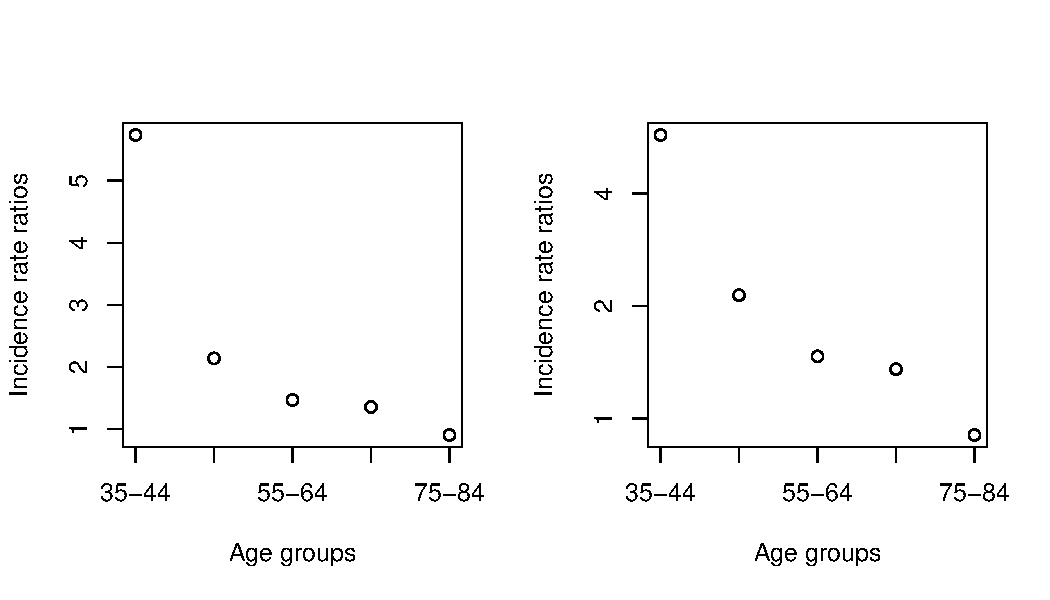
\includegraphics[width=\maxwidth]{figure/IRR_plot-1} \caption{\label{fig:IRR_plot}Plots of the incidence rate ratios depending on the age range.The graph on the left is in linear scale, while the graph on the right is on logarithmic scale.}\label{fig:IRR_plot}
\end{figure}

\end{knitrout}
  \item According to Figure \ref{fig:IRR_plot}:
  \begin{enumerate}
    \item Is the rate ratio greater than 1 for all age groups? What does it mean?
    \newline 
    No, it is not. In both plots, age group 75-84 is less than 1. Such as we know, a rate ratio greater than 1 indicates an increased risk
    for the group, and a rate ratio less than 1 indicates a decreased risk for the group. So, what it means that 75-84 age group has less risk than
    the others ages groups.
    \item Is the rate ratio constant over age groups? What does it mean?
    \newline
    No, it is not. This means that it is correlated with the age.
  \end{enumerate}
\end{enumerate}


%%%%%%%%%%%%%%%
%%%
%%% Section: Modeling incidence rates with a Generalized Linear Model
%%%
%%%%%%%%%%%%%%%
\section{Modeling incidence rates with a Generalized Linear Model}
\label{sec:Modelling}
Suppose we are interested in modeling the coronary deaths rate, $I = \frac{I}{\Delta t}$, where \textit{I} is the coronary deaths count and $\Delta t$ is follow-up (in person-years), as a function of smoking status (\textit{E}), which is the exposure of interest, and age group (\textit{A}). We suspect that smoking status could interact with age in the effect on coronary mortality. Hence, we consider the Generalized Linear Model (GLM) \footnote{You can find the \LaTeX code to write model \eqref{eq:model} in the file \Robject{model.tex.}} specified in equations \eqref{eq:model} to model the coronary deaths rate for individuals with smoking status \textit{i} and in age group \textit{j}, $I_{r_{ij}}$ :

\begin{equation}
\label{eq:model}
\left\{
\begin{array}{l}
\bullet\ \text{Probability distribution:} \\ \\
%%%%%%%%%%%%%%%%%%%%%%%%%%%%%%%%%%%%%%%%%
\qquad
I_{r_{ij}} = \frac{I_{ij}}{\Delta t_{ij}},
\qquad
%%%%%%%%%%%%%%%%%%%%%%%%%%%%%%%%%%%%%%%%%
I_{ij} \sim  \text{Pois}(\lambda_{ij}),
\qquad
%%%%%%%%%%%%%%%%%%%%%%%%%%%%%%%%%%%%%%%%%
\Delta t_{ij}\text{ is the follow-up;}\\ \\
%%%%%%%%%%%%%%%%%%%%%%%%%%%%%%%%%%%%%%%%%
\bullet\ \text{Model for the mean:} \\ \\
%%%%%%%%%%%%%%%%%%%%%%%%%%%%%%%%%%%%%%%%%
\qquad
\log
\left( \frac{\lambda_{ij}}{\Delta t_{ij}} \right) = L(E_i, A_j) \text{ (the linear predictor)}\\ \\
%%%%%%%%%%%%%%%%%%%%%%%%%%%%%%%%%%%%%%%%%
\qquad
L(E_i, A_j) = \alpha + \beta_i E_i + \gamma_j A_j + \delta_{ij} E_i A_j\\
%%%%%%%%%%%%%%%%%%%%%%%%%%%%%%%%%%%%%%%%%
\phantom{
\qquad
L(E_i, A_j)} = \alpha + \\
%%%
\phantom{
\qquad
L(E_i, A_j)} + \beta_1 \mathbbm{1}_{i=1} + \\
%%%
\phantom{
\qquad
L(E_i, A_j)
} + 
\gamma_1 \mathbbm{1}_{j=1} +
\gamma_2 \mathbbm{1}_{j=2} +
\gamma_3 \mathbbm{1}_{j=3} +
\gamma_4 \mathbbm{1}_{j=4} +\\
%%%
\phantom{
\qquad
L(E_i, A_j)
} + 
\delta_{11} \mathbbm{1}_{i=1}\mathbbm{1}_{j=1} +
\delta_{12} \mathbbm{1}_{i=1}\mathbbm{1}_{j=2} +
\delta_{13} \mathbbm{1}_{i=1}\mathbbm{1}_{j=3} +
\delta_{14} \mathbbm{1}_{i=1}\mathbbm{1}_{j=4},
\end{array}
\right.
\end{equation}
where
\begin{equation*}
\mathbbm{1}_{x=a}
=
\left\{
\begin{array}{ll}
1, & \text{if } x = a \\
0, & \text{if } x \neq a
\end{array}
\right..
\end{equation*}

Note that $I_{r_{ij}}$ is a random variable (different individuals with same smoke status and age can suffer or not coronary death within the same follow-up). Hence, the aim of fitting model \eqref{eq:model} is to estimate the expectation (i.e. mean) of the coronary deaths rate as:
\begin{equation*}
    \mathbb{E}(I_{r_{ij}}) =  \mathbb{E}\left(\frac{I_{ij}}{\Delta t_{ij}}\right) = \frac{\mathbb{E}(I_{ij})}{\Delta t_{ij}} = \frac{\lambda_{ij}}{\Delta t_{ij}} = \text{exp}(L(E_{i},A_{j})).
\end{equation*}

\begin{enumerate}
  \item Note that the logarithm function in model \eqref{eq:model} implies that we are assuming that the incidence rate varies exponentially with age. Is it         consistent with Figure \ref{fig:IRR_plot}? Why?

No, it is not consistent with Figure \ref{fig:IRR_plot}. At first, might seem that on the left plot there is plotted an exponential function.           Nevertheless, on the right plot, which is the same function plotted on the log-linear scale, there should be a straight line which clearly it is not.

  \item Prove that, under model \eqref{eq:model}, the expected IRR for smokers vs nonsmokers, for a given age group j is:
  
\begin{equation}
\label{eq:equation2}
        IRR_{j} = \begin{cases} \text{exp}(\beta_1), & \mbox{if $j = 0$,} \\ \text{exp}(\beta_1 + \delta_{1j}), & \mbox{if $j \not= 0$.} \end{cases}
\end{equation}
\textbf{Proof:}

\begin{flalign}
\label{eq:E(IRR)}
    &\mathbb{E}(IRR_{j}) =  \mathbb{E}\left(\frac{I_{r_{1j}}}{I_{r_{0j}}}\right) =  \frac{\mathbb{E}(I_{r_{1j}})}{\mathbb{E}(I_{r_{0j}})} = \begin{cases} (I), & \mbox{if $j = 0$,} \\ (II), & \mbox{if $j \not= 0$.} \end{cases} &
\end{flalign}
Where,
\begin{flalign}
    &(I) = \frac{\text{exp}(\alpha+\beta_{1}+0+0)}{\text{exp}(\alpha+0+0+0)} = \text{exp}(\alpha + \beta_{1} - \alpha) = \text{exp}(\beta_{1})&
\end{flalign}
\begin{flalign}
    (II) &= \frac{\displaystyle \text{exp}(\alpha + \beta_{1} + \sum_{k=1}^{4} \gamma_{k}\mathbbm{1}_{j=k} + \displaystyle \sum_{k=1}^{4} \delta_{1k}\mathbbm{1}_{j=k})}{ \displaystyle \text{exp}(\alpha + 0 + \sum_{k=1}^{4} \gamma_{k}\mathbbm{1}_{j=k} + 0)} &\\
    &= \displaystyle \text{exp}(\alpha + \beta_{1} + \sum_{k=1}^{4} \gamma_{k}\mathbbm{1}_{j=k} + \sum_{k=1}^{4} \delta_{1k}\mathbbm{1}_{j=k} - \alpha - \displaystyle \sum_{k=1}^{4} \gamma_{k}\mathbbm{1}_{j=k}) \notag&\\
    &= \text{exp}(\beta_{1} + \delta_{1j})\notag &
\end{flalign}


Hence, 
\begin{equation}
        \mathbb{E}(IRR_{j}) = \begin{cases} \text{exp}(\beta_{1}), & \mbox{if $j = 0$,} \\ \text{exp}(\beta_{1} + \delta_{1j}), & \mbox{if $j \not= 0$.} \end{cases}\\
\end{equation}
\QEDB
\item According to Figure \ref{fig:IRR_plot}, explain what sign (i.e. positive, negative or zero) do you
expect for $\delta_{1j}$.

In Figure \ref{fig:IRR_plot} we can see that both graphics are decreasing. That means that, if we increase the age groups (i.e. \textit{j} value), IRR decreases. If $j = 0$, we do not have any $\delta_{1j}$ value, which is equivalent to saying that $\delta_{1j} = 0$. Therefore, $\delta_{1j}$ has to be negative when $j > 0$ to make IRR value decrease. In fact, $\delta_{1j}$ will have lower values as \textit{j} becomes larger.

\item Model \eqref{eq:model} can be fitted in \textsf{R} as:
\begin{knitrout}\footnotesize
\definecolor{shadecolor}{rgb}{0.969, 0.969, 0.969}\color{fgcolor}\begin{kframe}
\begin{alltt}
\hlstd{> }\hlstd{mod} \hlkwb{<-} \hlkwd{glm}\hlstd{(deaths} \hlopt{~} \hlstd{smoker} \hlopt{*} \hlstd{age} \hlopt{+} \hlkwd{offset}\hlstd{(}\hlkwd{log}\hlstd{(personYears)),}
\hlstd{+ }           \hlkwc{family} \hlstd{= poisson,}
\hlstd{+ }           \hlkwc{data} \hlstd{= breslow)}
\end{alltt}
\end{kframe}
\end{knitrout}

that provides the following results:

\begin{knitrout}\footnotesize
\definecolor{shadecolor}{rgb}{0.969, 0.969, 0.969}\color{fgcolor}\begin{kframe}
\begin{alltt}
\hlstd{> }\hlkwd{summary}\hlstd{(mod)}
\end{alltt}
\begin{verbatim}
## 
## Call:
## glm(formula = deaths ~ smoker * age + offset(log(personYears)), 
##     family = poisson, data = breslow)
## 
## Deviance Residuals: 
##  [1]  0  0  0  0  0  0  0  0  0  0
## 
## Coefficients:
##                    Estimate Std. Error z value Pr(>|z|)    
## (Intercept)          -9.148      0.707  -12.94  < 2e-16 ***
## smokeryes             1.747      0.729    2.40    0.017 *  
## age45-54              2.357      0.764    3.09    0.002 ** 
## age55-64              3.830      0.732    5.23  1.7e-07 ***
## age65-74              4.623      0.732    6.32  2.7e-10 ***
## age75-84              5.294      0.730    7.26  4.0e-13 ***
## smokeryes:age45-54   -0.987      0.790   -1.25    0.212    
## smokeryes:age55-64   -1.363      0.756   -1.80    0.072 .  
## smokeryes:age65-74   -1.442      0.757   -1.91    0.057 .  
## smokeryes:age75-84   -1.847      0.757   -2.44    0.015 *  
## ---
## Signif. codes:  0 '***' 0.001 '**' 0.01 '*' 0.05 '.' 0.1 ' ' 1
## 
## (Dispersion parameter for poisson family taken to be 1)
## 
##     Null deviance:  9.3507e+02  on 9  degrees of freedom
## Residual deviance: -7.9936e-15  on 0  degrees of freedom
## AIC: 75.07
## 
## Number of Fisher Scoring iterations: 3
\end{verbatim}
\end{kframe}
\end{knitrout}


\item According the the fitted model, complete the following list \textbf{(using} \verb+\Sexpr+ \textbf{in your \Robject{Rnw} document)}:
\begin{itemize}
    \item $\hat{\alpha}$ = -9.15
    \item $\hat{\beta_{1}}$ = 1.75
    \item $\hat{\gamma_{1}}$ = 2.36
    \item $\hat{\gamma_{2}}$ = 3.83
    \item $\hat{\gamma_{3}}$ = 4.62
    \item $\hat{\gamma_{4}}$ = 5.29
    \item $\hat{\delta_{1}}$ = -0.99
    \item $\hat{\delta_{2}}$ = -1.36
    \item $\hat{\delta_{3}}$ = -1.44
    \item $\hat{\delta_{4}}$ = -1.85
\end{itemize}

\item Use formula \ref{eq:equation2} and estimates provided by \verb+summary(mod)+ to complete the following list \textbf{(using} \verb+\Sexpr+ \textbf{in your \Robject{Rnw} document)}:
\begin{itemize}
    \item $\widehat{IRR}_{35-44}$ = 1.75
    \item $\widehat{IRR}_{45-54}$ = 0.76
    \item $\widehat{IRR}_{55-64}$ = 0.38
    \item $\widehat{IRR}_{65-74}$ = 0.3
    \item $\widehat{IRR}_{75-84}$ = -0.1
\end{itemize}

\item Solve again questions 2. and 3. (only (a), (b) and (c)) in Section \ref{sec:Comparing_incidence_rates}, but using now model \eqref{eq:model}, formula \ref{eq:equation2} and coefficients estimates provided by \verb+summary(mod)+.

\begin{knitrout}\footnotesize
\definecolor{shadecolor}{rgb}{0.969, 0.969, 0.969}\color{fgcolor}\begin{kframe}
\begin{alltt}
\hlstd{> }\hlstd{alpha} \hlkwb{<-} \hlstd{mod}\hlopt{$}\hlstd{coefficients[[}\hlstr{'(Intercept)'}\hlstd{]]}
\hlstd{> }\hlstd{beta1} \hlkwb{<-} \hlstd{mod}\hlopt{$}\hlstd{coefficients[[}\hlstr{'smokeryes'}\hlstd{]]}
\hlstd{> }\hlstd{gamma1} \hlkwb{<-} \hlstd{mod}\hlopt{$}\hlstd{coefficients[[}\hlstr{'age45-54'}\hlstd{]]}
\hlstd{> }\hlstd{gamma4} \hlkwb{<-} \hlstd{mod}\hlopt{$}\hlstd{coefficients[[}\hlstr{'age75-84'}\hlstd{]]}
\hlstd{> }\hlstd{delta1} \hlkwb{<-} \hlstd{mod}\hlopt{$}\hlstd{coefficients[[}\hlstr{'smokeryes:age45-54'}\hlstd{]]}
\hlstd{> }\hlstd{delta4} \hlkwb{<-} \hlstd{mod}\hlopt{$}\hlstd{coefficients[[}\hlstr{'smokeryes:age75-84'}\hlstd{]]}
\hlstd{> }
\hlstd{> }
\hlstd{> }\hlstd{Ir_45Nonsmoker_model} \hlkwb{<-} \hlkwd{exp}\hlstd{(alpha} \hlopt{+} \hlstd{gamma1)}\hlopt{*}\hlnum{1000}
\hlstd{> }\hlstd{Ir_45smoker_model} \hlkwb{<-} \hlkwd{exp}\hlstd{(alpha} \hlopt{+} \hlstd{beta1} \hlopt{+} \hlstd{gamma1} \hlopt{+} \hlstd{delta1)}\hlopt{*}\hlnum{1000}
\hlstd{> }\hlstd{Ir_75Nonsmoker_model} \hlkwb{<-} \hlkwd{exp}\hlstd{(alpha} \hlopt{+} \hlstd{gamma4)}\hlopt{*}\hlnum{1000}
\hlstd{> }\hlstd{Ir_75smoker_model} \hlkwb{<-} \hlkwd{exp}\hlstd{(alpha} \hlopt{+} \hlstd{beta1} \hlopt{+} \hlstd{gamma4} \hlopt{+} \hlstd{delta4)}\hlopt{*}\hlnum{1000}
\hlstd{> }
\hlstd{> }\hlstd{IRR_45_model} \hlkwb{<-} \hlkwd{exp}\hlstd{(beta1} \hlopt{+} \hlstd{delta1)}
\hlstd{> }\hlstd{IRR_75_model} \hlkwb{<-} \hlkwd{exp}\hlstd{(beta1} \hlopt{+} \hlstd{delta4)}
\end{alltt}
\end{kframe}
\end{knitrout}
  \begin{enumerate}
    \item The estimated values, for the age group of 45 to 54 years old are:
      \begin{enumerate}
        \item The incidence rate among smokers was 2.4 coronary deaths a year per 1000 people.
        \item The incidence rate among nonsmokers was 1.12 coronary deaths a year per 1000 people.
        \item The incidence rate ratio was 2.14.
      \end{enumerate}
    \item The estimated values, for the age group of 75 to 84 years old are:
    \begin{enumerate}
      \item The incidence rate among smokers was 19.18 coronary deaths a year per 1000 people.
      \item The incidence rate among nonsmokers was 21.2 coronary deaths a year per 1000 people.
      \item The incidence rate ratio was 0.9.
    \end{enumerate}
  \end{enumerate}

\end{enumerate}


%%%%%%%%%%%%%%%
%%%
%%% Section: Discussion
%%%
%%%%%%%%%%%%%%%
\section{Discussion}
\label{sec:discussion}
Based on the results of this analysis of the \Robject{breslow} data, discuss, in no more than 10 lines, about if smoking is a risk factor for coronary artery disease. Specifically, take into account concepts such as data context, modeling approach, confusion and interaction:

The Wald tests' p-values executed in questions 2.2.e and 2.3.e. suggest a possible association between coronary artery disease and smoking among the younger demographics of our population. Observing Table \ref{tab:table2} it is visible that the incidence rate of coronary artery disease increases with age, but the association between said incidence rate and smoking decreases with age too. This makes sense to us because we suspect that older people are more likely to die of coronary death. It should be taken into account, however, that this analysis was performed on data from male doctors, and thus, generalizing the results for the general population might not be accurate. An interesting ampliation of the experiment would be to perform the same tests on a balanced dataset with individuals of different sexes, social backgrounds and economical statuses.

%%%%%%%%%%%%%%%
%%%
%%% References
%%%
%%%%%%%%%%%%%%%
\begin{thebibliography}{99}

\bibitem{ref1}Doll R, Hill A.B. Mortality of British doctors in relation to smoking: Observations on coronary thrombosis. National Cancer Institute Monograph. 1966;19:205-268.

\bibitem{ref2}Breslow N.E. Cohort Analysis in Epidemiology. In A Celebration of Statistics A.C.Atkinson and S.E. Fienberg (editors). 1985;109-143. Springer-Verlag.

\end{thebibliography}


%%%%%%%%%%%%%%%
%%%
%%% Appendix
%%%
%%%%%%%%%%%%%%%
\clearpage


\appendix
\section{R code}
\label{app:Rcode}

\subsection{Libraries used, data load and, $I_{r_{ij}}$ and $IRR_{j}$ implementation.}
\label{app:Ir and IRR}

\begin{knitrout}\footnotesize
\definecolor{shadecolor}{rgb}{0.969, 0.969, 0.969}\color{fgcolor}\begin{kframe}
\begin{alltt}
\hlstd{> }\hlcom{### libraries used:}
\hlstd{> }\hlkwd{library}\hlstd{(knitr)}
\hlstd{> }\hlkwd{library}\hlstd{(highlight)}  \hlcom{# to highlight R output}
\hlstd{> }\hlkwd{library}\hlstd{(xtable)}     \hlcom{# to export R output tables to LaTeX}
\hlstd{> }\hlkwd{library}\hlstd{(here)}
\hlstd{> }\hlkwd{library}\hlstd{(mice)}
\hlstd{> }\hlkwd{library}\hlstd{(plotrix)}
\hlstd{> }\hlkwd{library}\hlstd{(epitools)}
\hlstd{> }\hlkwd{library}\hlstd{(kableExtra)}
\hlstd{> }
\hlstd{> }\hlkwd{set.seed}\hlstd{(}\hlnum{1936}\hlstd{)}
\end{alltt}
\end{kframe}
\end{knitrout}



\begin{knitrout}\footnotesize
\definecolor{shadecolor}{rgb}{0.969, 0.969, 0.969}\color{fgcolor}\begin{kframe}
\begin{alltt}
\hlstd{> }\hlcom{# Ir implementation }
\hlstd{> }\hlstd{Ir_smokers} \hlkwb{<-} \hlstd{Data}\hlopt{$}\hlstd{deaths[Data}\hlopt{$}\hlstd{smoker}\hlopt{==}\hlstr{'yes'}\hlstd{]}\hlopt{/}\hlstd{Data}\hlopt{$}\hlstd{personYears[Data}\hlopt{$}\hlstd{smoker}\hlopt{==}\hlstr{'yes'}\hlstd{]}\hlopt{*}\hlnum{1000}
\hlstd{> }\hlstd{Ir_Nonsmokers} \hlkwb{<-} \hlstd{Data}\hlopt{$}\hlstd{deaths[Data}\hlopt{$}\hlstd{smoker}\hlopt{==}\hlstr{'no'}\hlstd{]}\hlopt{/}\hlstd{Data}\hlopt{$}\hlstd{personYears[Data}\hlopt{$}\hlstd{smoker}\hlopt{==}\hlstr{'no'}\hlstd{]}\hlopt{*}\hlnum{1000}
\end{alltt}
\end{kframe}
\end{knitrout}

\begin{knitrout}\footnotesize
\definecolor{shadecolor}{rgb}{0.969, 0.969, 0.969}\color{fgcolor}\begin{kframe}
\begin{alltt}
\hlstd{> }\hlcom{# IRR implementation}
\hlstd{> }\hlstd{IRR} \hlkwb{<-} \hlstd{Ir_smokers}\hlopt{/}\hlstd{Ir_Nonsmokers}
\end{alltt}
\end{kframe}
\end{knitrout}

\subsection{Implementation of sentences results for age group 45-54.}
\label{app:IncidenceRates2}
\begin{knitrout}\footnotesize
\definecolor{shadecolor}{rgb}{0.969, 0.969, 0.969}\color{fgcolor}\begin{kframe}
\begin{alltt}
\hlstd{> }\hlcom{# The incidence rate among smokers}
\hlstd{> }\hlstd{Ir_45smoker} \hlkwb{<-} \hlstd{Ir_smokers[}\hlnum{2}\hlstd{]} \hlcom{# coronary deaths a year per 1000 people}
\hlstd{> }
\hlstd{> }\hlcom{# The incidence rate among nonsmokers}
\hlstd{> }\hlstd{Ir_45Nonsmoker} \hlkwb{<-} \hlstd{Ir_Nonsmokers[}\hlnum{2}\hlstd{]} \hlcom{# coronary deaths a year per 1000 people}
\hlstd{> }
\hlstd{> }\hlcom{# The incidence rate ratio}
\hlstd{> }\hlstd{IRR_45} \hlkwb{<-} \hlstd{Ir_45smoker}\hlopt{/}\hlstd{Ir_45Nonsmoker} \hlcom{# rate (no units, since it's a dimensionless magnitude)}
\hlstd{> }
\hlstd{> }\hlcom{# The p-value of the Wald test}
\hlstd{> }\hlstd{Data45} \hlkwb{<-} \hlstd{Data[Data}\hlopt{$}\hlstd{age}\hlopt{==}\hlstr{"45-54"}\hlstd{,]}
\hlstd{> }\hlstd{pValue45} \hlkwb{<-} \hlkwd{rateratio.wald}\hlstd{(}\hlkwc{x}\hlstd{=Data45}\hlopt{$}\hlstd{deaths,}\hlkwc{y}\hlstd{=Data45}\hlopt{$}\hlstd{personYears,)}\hlopt{$}\hlstd{p.value[}\hlnum{2}\hlstd{,}\hlstr{"wald"}\hlstd{]}
\end{alltt}
\end{kframe}
\end{knitrout}

\subsection{Implementation of sentences results for age group 75-84.}
\label{app:IncidenceRates3}
\begin{knitrout}\footnotesize
\definecolor{shadecolor}{rgb}{0.969, 0.969, 0.969}\color{fgcolor}\begin{kframe}
\begin{alltt}
\hlstd{> }\hlcom{# The incidence rate among smokers}
\hlstd{> }\hlstd{Ir_75smoker} \hlkwb{<-} \hlstd{Ir_smokers[}\hlnum{5}\hlstd{]} \hlcom{# coronary deaths a year per 1000 people}
\hlstd{> }
\hlstd{> }\hlcom{# The incidence rate among nonsmokers}
\hlstd{> }\hlstd{Ir_75Nonsmoker} \hlkwb{<-} \hlstd{Ir_Nonsmokers[}\hlnum{5}\hlstd{]} \hlcom{# coronary deaths a year per 1000 people}
\hlstd{> }
\hlstd{> }\hlcom{# The incidence rate ratio}
\hlstd{> }\hlstd{IRR_75} \hlkwb{<-} \hlstd{Ir_75smoker}\hlopt{/}\hlstd{Ir_75Nonsmoker} \hlcom{# rate (no units, since it is dimensionless)}
\hlstd{> }
\hlstd{> }\hlcom{# The p-value of the Wald test}
\hlstd{> }\hlstd{Data75} \hlkwb{<-} \hlstd{Data[Data}\hlopt{$}\hlstd{age}\hlopt{==}\hlstr{"75-84"}\hlstd{,]}
\hlstd{> }\hlstd{pValue75} \hlkwb{<-} \hlkwd{rateratio.wald}\hlstd{(}\hlkwc{x}\hlstd{=Data75}\hlopt{$}\hlstd{deaths,}\hlkwc{y}\hlstd{=Data75}\hlopt{$}\hlstd{personYears,)}\hlopt{$}\hlstd{p.value[}\hlnum{2}\hlstd{,}\hlstr{"wald"}\hlstd{]}
\end{alltt}
\end{kframe}
\end{knitrout}

\subsection{Implementation of Figure \ref{fig:IRR_plot}.}
\label{app:IRR_plot}
\begin{knitrout}\footnotesize
\definecolor{shadecolor}{rgb}{0.969, 0.969, 0.969}\color{fgcolor}\begin{kframe}
\begin{alltt}
\hlstd{> }\hlcom{# Division of space into two plots}
\hlstd{> }\hlkwd{par}\hlstd{(}\hlkwc{mfrow} \hlstd{=} \hlkwd{c}\hlstd{(}\hlnum{1}\hlstd{,} \hlnum{2}\hlstd{))}
\hlstd{> }
\hlstd{> }\hlcom{# IRR plot in linear scale}
\hlstd{> }\hlkwd{plot}\hlstd{(IRR,} \hlkwc{xaxt} \hlstd{=} \hlstr{'n'}\hlstd{,} \hlkwc{xlab} \hlstd{=} \hlstr{'Age groups'}\hlstd{,} \hlkwc{ylab} \hlstd{=} \hlstr{'Incidence rate ratios'}\hlstd{)}
\hlstd{> }\hlkwd{axis}\hlstd{(}\hlnum{1}\hlstd{,} \hlkwc{at} \hlstd{=} \hlkwd{seq}\hlstd{(}\hlnum{1}\hlstd{,} \hlnum{5}\hlstd{),} \hlkwc{labels} \hlstd{=} \hlkwd{c}\hlstd{(}\hlstr{'35-44'}\hlstd{,} \hlstr{'45-54'}\hlstd{,} \hlstr{'55-64'}\hlstd{,} \hlstr{'65-74'}\hlstd{,} \hlstr{'75-84'}\hlstd{))}
\hlstd{> }
\hlstd{> }\hlcom{# IRR plot in logarithmic scale}
\hlstd{> }\hlkwd{plot}\hlstd{(}\hlkwc{log} \hlstd{=} \hlstr{'y'}\hlstd{, IRR,} \hlkwc{xaxt} \hlstd{=} \hlstr{'n'}\hlstd{,} \hlkwc{yaxt} \hlstd{=} \hlstr{'n'} \hlstd{,} \hlkwc{xlab} \hlstd{=} \hlstr{'Age groups'}\hlstd{,}
\hlstd{+ }     \hlkwc{ylab} \hlstd{=} \hlstr{'Incidence rate ratios'}\hlstd{,} \hlkwc{ylim} \hlstd{=} \hlkwd{c}\hlstd{(}\hlkwd{min}\hlstd{(IRR),} \hlkwd{max}\hlstd{(IRR)))}
\hlstd{> }\hlkwd{axis}\hlstd{(}\hlnum{1}\hlstd{,} \hlkwc{at} \hlstd{=} \hlkwd{seq}\hlstd{(}\hlnum{1}\hlstd{,} \hlnum{5}\hlstd{),} \hlkwc{labels} \hlstd{=} \hlkwd{c}\hlstd{(}\hlstr{'35-44'}\hlstd{,} \hlstr{'45-54'}\hlstd{,} \hlstr{'55-64'}\hlstd{,} \hlstr{'65-74'}\hlstd{,} \hlstr{'75-84'}\hlstd{))}
\hlstd{> }\hlstd{ylabels} \hlkwb{<-} \hlnum{2}\hlopt{^}\hlkwd{seq}\hlstd{(}\hlnum{0}\hlstd{,} \hlkwd{as.integer}\hlstd{(}\hlkwd{log}\hlstd{(}\hlkwd{max}\hlstd{(IRR),} \hlnum{2}\hlstd{)))}
\hlstd{> }\hlkwd{axis}\hlstd{(}\hlnum{2}\hlstd{,} \hlkwc{at} \hlstd{= ylabels,} \hlkwc{labels} \hlstd{= ylabels)}
\end{alltt}
\end{kframe}
\end{knitrout}



\end{document}
